172. \begin{figure}[ht!]
\center{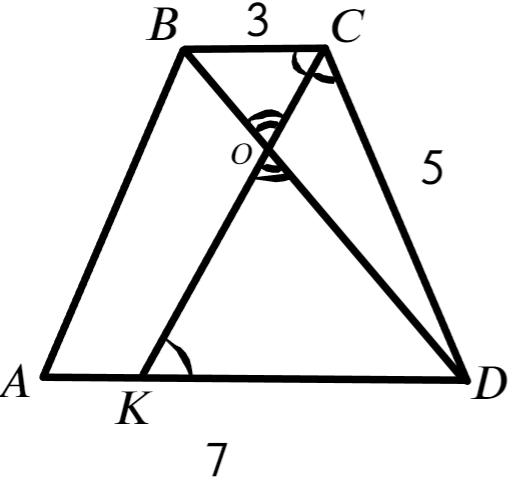
\includegraphics[scale=0.35]{g9-172.png}}
\end{figure}\\
Так как $CK$ --- биссектриса, а углы $BCO$ и $OKD$ являются накрест лежащими при параллельных прямых $AD$ и $BC,$ имеем равенства $\angle DCK=\angle BCO=\angle OKD,$ поэтому треугольник $DCK$ является равнобедренным и $DK=CD=5.$ $\angle BOC=\angle KOD$ как вертикальные, а $\angle BCO=\angle OKD$ как накрест лежащие, значит треугольники $BOC$ и $KOD$ подобны (по двум углам) с коэффициентом $\cfrac{BC}{KD}=\cfrac{3}{5}.$ Высота трапеции равна $2\cdot\cfrac{20}{3+7}=4.$ Если высота треугольника $BOC$ равна $x,$ то высота треугольника $KOD$ равна $\cfrac{5}{3}x$ и $x+\cfrac{5}{3}x=4,\ \cfrac{8}{3} x=4,\ x=\cfrac{3}{2}.$ Тогда $S_{\Delta BOC}=\cfrac{1}{2}\cdot\cfrac{3}{2}\cdot3=\cfrac{9}{4}.$
ewpage
oindent
